\documentclass[a4paper]{scrartcl}
\usepackage[]{hyperref}
\usepackage{graphicx}
\begin{document}

\title{Supervised Learning: Classification and Regression}
\subtitle{Titanic Passenger List}
\author{Ronan McHugh s162927}

\maketitle

\section{Introduction}
\paragraph{}
In this paper I present the outcome of a regression problem and a classification problem on the dataset \textbf{Titanic Passenger List} as provided by Kaggle.com\cite{kaggle16}. For the regression problem I chose to predict \emph{Fare}, while for the classification problem I chose to predict \emph{Survival}.
\subsection{Feature engineering and data transformations}
\paragraph{}
For this assignment I decided to improve the dataset through feature engineering. 
Following the example of Risdal\cite{risdal16}, I created two new features, \emph{Title} and \emph{FamilySize}. In addition, I performed data cleaning on the \emph{Fare} attribute and the \emph{Age} attribute.

\subparagraph{Title} 
\emph{Title} was created by extracting passenger title from the \emph{Name} attribute. The \emph{Name} attribute is well structured and always contains a title of some sort. These titles can be indicative of a passenger's age, sex, marital status, profession and social status and as such can be assumed to be of relevance in determining their fare (in the case of regression).
Creating the attribute was a simple matter of identifying all possible values and parsing these out from the text of the name attribute. 

\subparagraph{FamilySize} \emph{FamilySize} was created  by combining the \emph{Parch} and \emph{SibSp} attributes for each passenger. This gave a count for the total number of family members travelling with the passenger.

\subparagraph{Fare} 
As discussed in our previous report, the \emph{Fare} attribute is extremely noisy\cite{chegmch16}. After examining the values in the dataset and comparing them to information on actual ticket prices, I determined that many of the prices in the dataset were simply missing a decimal separator, for example, a passenger's fare might have the value 7925, when the actual value should be 7.925 \cite{ref16} \cite{enctit16}. Once I realised this, it was trivial to write a transformation to add the decimal point in the correct location before transforming the attribute to a numeric datatype. The outcome of this step is visualised in \ref{fig:cleaned_fare}.	  

\subparagraph{Age}
There are approx 177 observations that are missing the value for \emph{Age}. Since the engineered attribute \emph{Title} has some relevance to \emph{Age}, I decided to use the mean for that observation's title to fill in the  \emph{Age}variable. This was preferable to dropping the attribute as I presumed it had some significance for both the \emph{Fare} and the \emph{Survived} category.


\begin{figure}
  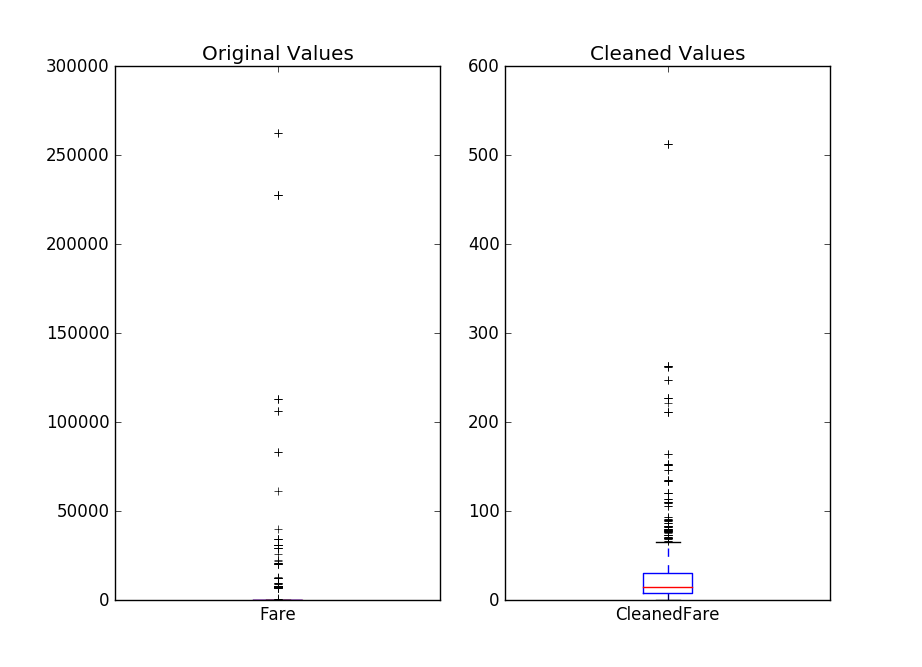
\includegraphics[scale=.42]{graphs/cleaned_fare.png}
  \centering  
  \caption{Distribution of Fare values before and after data cleaning. As can be seen, the cleaning process greatly reduces the range of the values in keeping with the historical data.}
  \label{fig:cleaned_fare}
\end{figure}

\subparagraph{}
The code for all these transformations can be seen in the \verb+titanic_data.py+ script in the GitHub repo\cite{ronanmch16}.

\section{Regression models}
\subsection{Target problem}
\paragraph{}
I chose to predict \emph{Fare} for two reasons: firstly, it is the only continuous attribute. There are other interval attributes such as \emph{Parch} (number of Parents or Children) and \emph{SibSp} (number of siblings) but these are discrete, i.e. they increase in intervals of one. Obviously we could round the results of a linear regression to return discrete values, but I preferred not to add this layer of processing for simplicity's sake. I also assumed that \emph{Fare} would be easier to predict based on other attributes such as \emph{Pclass} and \emph{Embarked}.

\subsection{Estimation method}
Before attempting to solve the regression problems, I wanted to compare the value of the two different cross validation methods, \emph{K-Fold} and \emph{Holdout}. To do this, I used forward selection to choose the model's predictor features, first using \emph{Holdout} to partition the dataset once, then using \emph{K-Fold} to test the model against \emph{K=3} different partitions, choosing a model based on the best average score. I then estimated the generalisation error by by testing the same models against a new section of the dataset that had not been tested. The results are shown in \ref{fig:holdout_vs_kfold}. The differences between the train and test errors in both figures demonstrates the effect of overfitting, as the generalisation error on the test set quickly increases as the model becomes more complex. Interestingly, the second feature chosen when using the forward select algorithm with \emph{Holdout} increased the generalisation error dramatically.  

\begin{figure}
  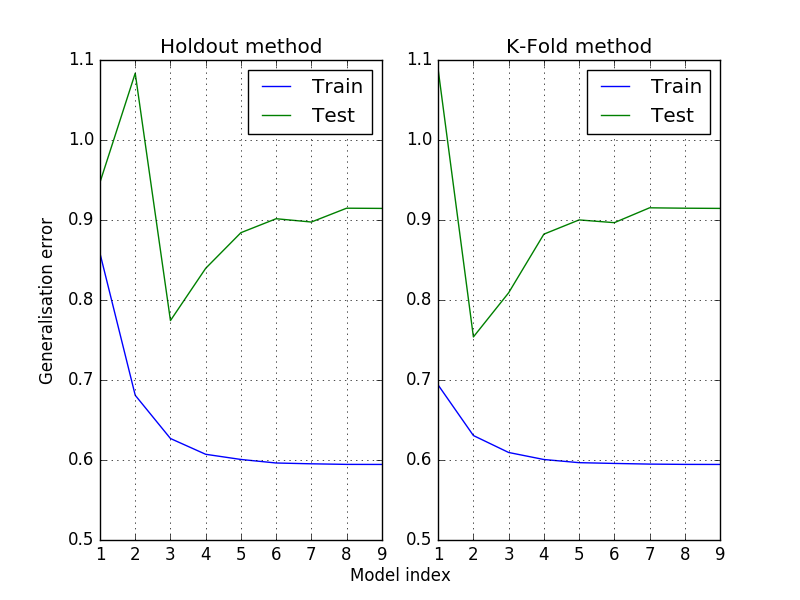
\includegraphics[scale=.3]{graphs/holdout_vs_kfold.png}
  \centering
  \caption{Two layer cross validation of a linear regression model selected using \emph{Holdout} and \emph{K-Fold} methods.}
  \label{fig:holdout_vs_kfold}
\end{figure}

\subsection{Linear Regression vs Artificial Neural Network}
My next step was to test the linear model against an artificial neural network. In both of these cases, the simpler models performed best, as shown in \ref{fig:regr_vs_neural}. The best model in both cases used \emph{Pclass} and \emph{FamilySize} attributes but the neural network achieved greater accuracy with these features than the linear regression model did.

\begin{center}
\begin{tabular}{| p{2cm} | p{6cm} | l | l |}
\hline
\textbf{Model no.} & \textbf{Features} & \textbf{Training Error} &\textbf{Generalisation Error} \\ \hline
1 & Pclass & 0.693668932859 & 1.08792303578 \\ \hline
2 & Pclass, FamilySize & 0.63056706974 & 0.75383547945 \\ \hline
3 & Pclass, FamilySize, EmbC & 0.609404541756 & 0.809015005427 \\ \hline
4 & Pclass, FamilySize, EmbC, TitMiss & 0.600616352988 & 0.882308006674 \\ \hline
5 & Pclass, FamilySize, EmbC, TitMiss, TitMr & 0.596669908103 & 0.900102154391 \\ \hline
6 & Pclass, FamilySize, EmbC, TitMiss, TitMr, EmbS & 0.59570952962 & 0.896667239259 \\ \hline
7 & Pclass, FamilySize, EmbC, TitMiss, TitMr, EmbS, Age & 0.594876034449 & 0.915238158019 \\ \hline
8 & Pclass, FamilySize, EmbC, TitMiss, TitMr, EmbS, Age, Sex & 0.594522619792 & 0.914746729854 \\ \hline
9 & Pclass, FamilySize, EmbC, TitMiss, TitMr, EmbS, Age, Sex, TitJonkheer & 0.594453353629 & 0.914495781798 \\ \hline

\end{tabular}
\end{center}

\begin{tabular}{| p{2cm} | p{6cm} | l | l |}
\hline
\textbf{Model no.} & \textbf{Features} & \textbf{Training Error} &\textbf{Generalisation Error} \\ \hline
1 & Pclass & 0.74298202346 & 1.00889994789 \\ \hline
2 & Pclass, FamilySize & 0.617927482288 & 0.676099756959 \\ \hline
3 & Pclass, FamilySize, EmbS & 0.580475408698 & 0.700400729806 \\ \hline
4 & Pclass, FamilySize, EmbS, TitMiss & 0.568710178287 & 0.814791319813 \\ \hline
5 & Pclass, FamilySize, EmbS, TitMiss, TitMajor & 0.563178953451 & 0.774113538632 \\ \hline
6 & Pclass, FamilySize, EmbS, TitMiss, TitMajor, EmbQ & 0.561266432856 & 0.831908571141 \\ \hline
\end{tabular}

\begin{figure}
  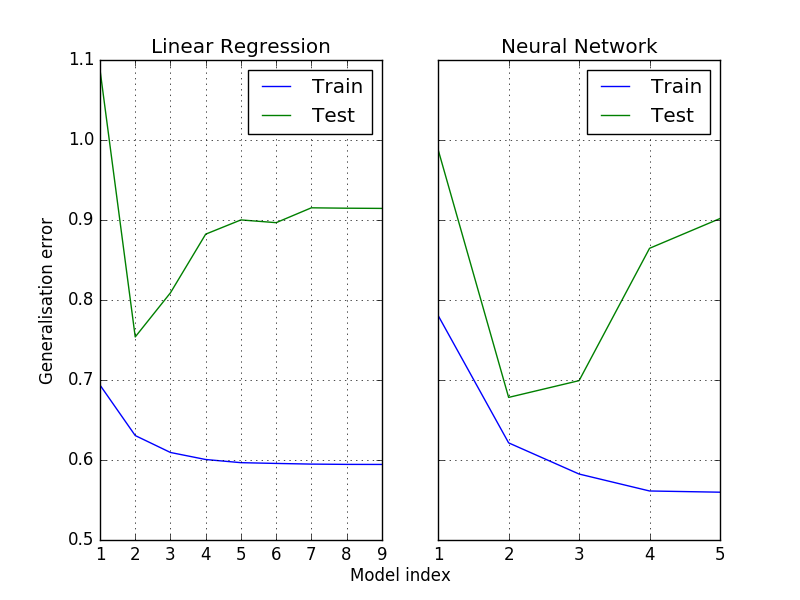
\includegraphics[scale=.3]{graphs/regr_vs_neural.png}
  \centering
  \caption{Two layer cross validation comparison of linear regression and artificial neural network.}
  \label{fig:regr_vs_neural}
\end{figure}

\section{Classification models}

\begin{thebibliography}{9}

\bibitem{kaggle16}
  Kaggle,
  \emph{Titanic: Machine Learning From Disaster},
  {\url{https://www.kaggle.com/c/titanic/}}
 
\bibitem{risdal16}
  Megan Risdal,
  \emph{Exploring the Titanic Dataset},
  {\url{https://www.kaggle.io/svf/198371/166ea2e9c1074ca9cd2447c7ee27cf10/__results__.html}}
  
\bibitem{ronanmch16}
  Ronan McHugh,
  \emph{Machine Learning},
  {\url{https://github.com/ronan-mch/machine_learning}}
  
\bibitem{chegmch16}
  Ali Chegini,
  Ronan McHugh,
  \emph{Feature Extraction and Visualisation - Introduction to Machine Learning - Project 1},
  {\url{https://docs.google.com/document/d/1QSV2kJBotRCUvSiBF7-Z3Jjz6BoKB2H9TaV4PGRheTk/edit?usp=sharing}}
  
\bibitem{ref16}
  Reference.com,
  \emph{What were the prices of Titanic Tickets in 1912?},
  {\url{https://www.reference.com/history/were-prices-titanic-tickets-1912-53fecb79d8634272}}
  
\bibitem{enctit16}
  Encylopedia Titanica,
  \emph{Titanic Passenger List},
  {\url{https://www.encyclopedia-titanica.org/titanic-passenger-list/}}
 


\end{thebibliography}

\end{document}